\documentclass[t]{beamer}
\mode<presentation>

\usepackage{etex}

\usetheme{Madrid}
% other themes: Warsaw, AnnArbor, Antibes, Bergen, Berkeley, Berlin, Boadilla, boxes, CambridgeUS, Copenhagen, Darmstadt, default, Dresden, Frankfurt, Goettingen,
% Hannover, Ilmenau, JuanLesPins, Luebeck, Madrid, Maloe, Marburg, Montpellier, PaloAlto, Pittsburg, Rochester, Singapore, Szeged, classic

\setbeamertemplate{navigation symbols}{\insertslidenavigationsymbol}

\usecolortheme{dolphin}
%\usecolortheme{seagull}
% color themes: albatross, beaver, beetle, crane, default, dolphin, dov, fly, lily, orchid, rose, seagull, seahorse, sidebartab, structure, whale, wolverine

%\usefonttheme{serif}
% font themes: default, professionalfonts, serif, structurebold, structureitalicserif, structuresmallcapsserif

% pdf is displayed in full screen mode automatically
%\hypersetup{pdfpagemode=FullScreen}

%\AtBeginSection[]
%{
%  \begin{frame}<beamer>
%    \frametitle{Outline}
%    \tableofcontents[currentsection,currentsubsection]
%  \end{frame}
%}

% define your own colours:
\definecolor{Red}{rgb}{1,0,0}
\definecolor{Blue}{rgb}{0,0,1}
\definecolor{Green}{rgb}{0,1,0}
\definecolor{magenta}{rgb}{1,0,.6}
\definecolor{lightblue}{rgb}{0,.8,1}
\definecolor{lightpurple}{rgb}{.6,.4,1}
\definecolor{gold}{rgb}{.6,.5,0}
\definecolor{orange}{rgb}{1,0.4,0}
\definecolor{hotpink}{rgb}{1,0,0.5}
\definecolor{newcolor2}{rgb}{.5,.3,.5}
\definecolor{newcolor}{rgb}{0,.3,1}
\definecolor{newcolor3}{rgb}{1,0,.35}
\definecolor{darkgreen1}{rgb}{0, .35, 0}
\definecolor{darkgreen}{rgb}{0, .6, 0}
\definecolor{darkred}{rgb}{.75,0,0}

\xdefinecolor{olive}{cmyk}{0.64,0,0.95,0.4}
\xdefinecolor{purpleish}{cmyk}{0.75,0.75,0,0}

%\usepackage{beamerinnerthemerounded}
% inner themes include circles, default, inmargin, rectangles, rounded

%\usepackage{beamerouterthemesmoothbars}
% outer themes include default, infolines, miniframes, shadow, sidebar, smoothbars, smoothtree, split, tree

\useoutertheme[subsection=false]{smoothbars}

% to have the same footer on all slides
\setbeamertemplate{footline}[text line]{
\raisebox{3pt}{
\includegraphics[height=15pt]{su-long.eps}}\hfill 
\raisebox{5pt}{Math 207:  Statistics}\hfill 
\raisebox{5pt}{Chance Errors in Sampling}\hfill
\raisebox{5pt}{\insertframenumber/\pageref{lastpage}}}
%\setbeamertemplate{footline}[text line]{} % or empty footer

% include packages
\usepackage{subfigure}
\usepackage{multicol}
\usepackage{amsmath}
\usepackage{epsfig}
\usepackage{graphicx}
\usepackage[all,knot]{xy}
\xyoption{arc}
\usepackage{url}
\usepackage{multimedia}
\usepackage{hyperref}
\usepackage{setspace}

\title{Math 207:  Statistics}
\subtitle{Chapter 20:  Chance Errors in Sampling}
\author{Ralph Wojtowicz}
\institute{Mathematics Department\\ Shenandoah University}
%\date{\scriptsize 17 February 2012}

\usepackage{pstricks,pst-grad,pst-func,pst-text,pst-node,multido,pst-plot,calc,pst-3dplot}

\newcommand{\BRACE}{
\begin{pspicture}(-3,-2.1)(3,1.1)
\psset{yunit=3,linewidth=0.02}
\psline(-3.5,0)(3.5,0)  
  \psline(-3,0)(-3,-0.04) \rput[t](-3,-0.07){\scriptsize -3\hphantom{-}}
  \psline(-2,0)(-2,-0.04) \rput[t](-2,-0.07){\scriptsize -2\hphantom{-}}
  \psline(-1,0)(-1,-0.04) \rput[t](-1,-0.07){\scriptsize -1\hphantom{-}}
  \psline(0,0)(0,-0.04)   \rput[t](0,-0.07){\scriptsize 0}
  \psline(1,0)(1,-0.04)   \rput[t](1,-0.07){\scriptsize 1}
  \psline(2,0)(2,-0.04)   \rput[t](2,-0.07){\scriptsize 2}
  \psline(3,0)(3,-0.04)   \rput[t](3,-0.07){\scriptsize 3}
  \rput[l](3.6,0){\scriptsize $x$}
\psline(0,0)(0,0.5)
  \psline(-0.12,0.5)(0,0.5)    \rput[r](-0.21,0.5){\scriptsize $0.5$}
  \psline(-0.12,0.25)(0,0.25)  \rput[r](-0.21,0.25){\scriptsize $0.25$}
\psGauss[linecolor=blue,linewidth=0.02,sigma=1,mue=0]{-3}{3}
\pnode(-1,-0.15){A}\pnode(1,-0.15){B}
\psbrace[braceWidth=0.02,braceWidthInner=5pt,braceWidthOuter=5pt](A)(B){\rput{90}(0.25,-0.05){\scriptsize 68\%}}
%
\pnode(-2,-0.15){C}\pnode(2,-0.15){D}
\psbrace[braceWidth=0.02,braceWidthInner=25pt,braceWidthOuter=5pt](C)(D){\rput{90}(0.25,-0.05){\scriptsize 95\%}}
%
\pnode(-3,-0.15){E}\pnode(3,-0.15){F}
\psbrace[braceWidth=0.02,braceWidthInner=45pt,braceWidthOuter=5pt](E)(F){\rput{90}(0.25,-0.1){\scriptsize 99.7\%}}
\end{pspicture}}

\begin{document}

%\frame[plain]{
%	\titlepage
%}


\begin{frame}[plain]
\definecolor{myblue}{rgb}{0,0,0.6}
\definecolor{grayA}{rgb}{0.95,0.95,0.95}
\definecolor{grayB}{rgb}{0.98,0.98,0.98}
\begin{center}

%\begin{pspicture}(0,0)(7,4.8)
\begin{pspicture}(-6,-7)(6,2)

%\rput(0,-1.85){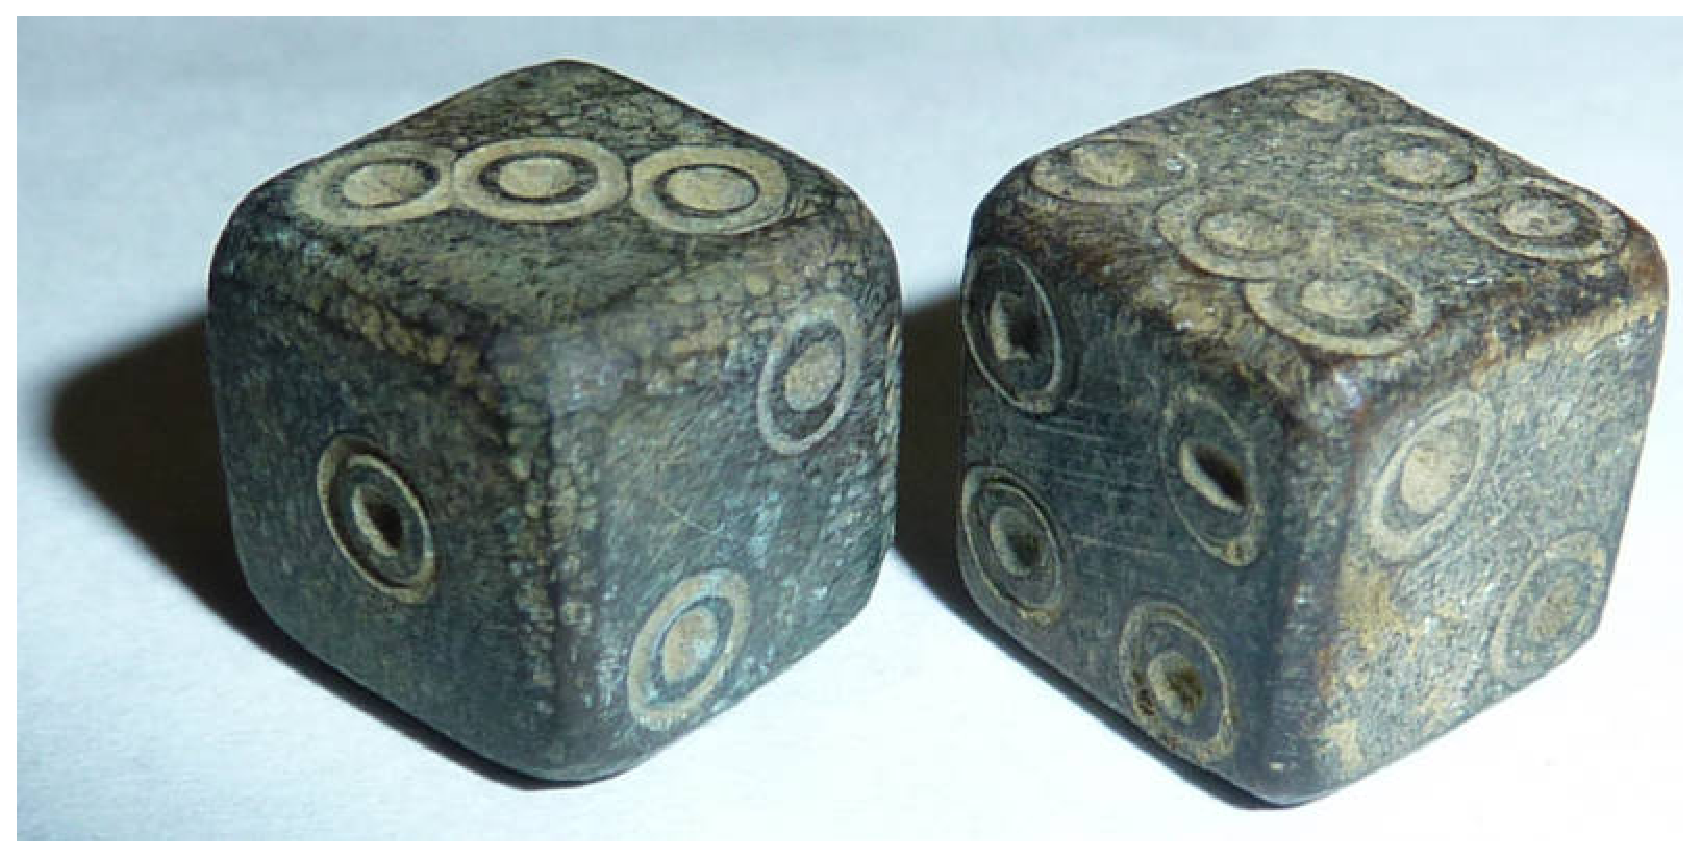
\includegraphics[height=4.2cm]{dice.eps}}
\psframe[linewidth=0.02,linecolor=gray](-6.2,-7)(6.2,2.2)
\psframe[linewidth=0.02,linecolor=gray](-6.15,-6.95)(6.15,2.15)
\rput(0,1.4){\color{myblue}\large Math 207:  Statistics}
\rput(0,0.6){\color{myblue}Chapter 20: Chance Error in Sampling}
%
\psframe[linewidth=0.02,fillstyle=solid,fillcolor=grayA](-2,-3)(2,-1)
  \rput[tl](-1.9,-1.1){\tiny Population (parameters)}
\psframe[linewidth=0.02,fillstyle=solid,fillcolor=grayB](-0.25,-2.75)(1.75,-2)
  \rput[tl](-0.15,-2.1){\tiny Sample (statistics)}
%\psframebox(0,0)(4,4)
\rput(0,-4.5){\scriptsize Dr.~Ralph Wojtowicz}
\rput(0,-5.0){\scriptsize Mathematics Department}
\rput(0,-5.8){
\includegraphics[height=1cm]{su-long.eps}}
%
%\rput(0,-6.5){\scriptsize 17 February 2012}
\end{pspicture}
\end{center}

\end{frame}

%\section[Outline]{}

\addtocounter{page}{-1}
\addtocounter{framenumber}{-1}

{\footnotesize
\frame{\tableofcontents}
}

\section{EV, SE and the Central Limit Theorem}

\begin{frame}
\frametitle{Expected Value, Standard Error,  Central Limit Theorem}
\begin{center}

\footnotesize

\begin{itemize}
\item Many statistics problems are modeled as  samples
   from a box of numbered tickets.
\item Solution procedure: 
   \begin{itemize}
   \item \scriptsize Formulate a box model.
   \item \scriptsize Compute the average and SD of the contents of the box.
   \item \scriptsize Determine if you are computing a sum or average (\%
      in a 0/1 box is an average).
   \item Use the appropriate formulas to compute the EV and SE
      for the sample.
   \item Use the normal curve  to compute chances of the 
      sample being in a specified range.
   \end{itemize}
\end{itemize}
%\begin{pspicture}(0,0)(7,4.8)
\begin{pspicture}(-6,-7)(6,0.2)
\rput(0.8, -1.4){
\begin{tabular}{cc}
\scalebox{0.65}{\begin{pspicture}(1.2,0)(11.3,4)
\psset{yunit=0.05, xunit=2.25}
\psline[linestyle=dotted](1,0)(4,0)
\rput[t](2.5,80){\textbf{Sum of Draws}}
\rput(2.5,65){$\mbox{EV}_{\mbox{\scriptsize sum}} = n\times\mbox{AV}_{\mbox{\scriptsize box}}$}
\rput(2.56,55){$\mbox{SE}_{\mbox{\scriptsize sum}} = \sqrt{n}\times\mbox{sd}_{\mbox{\scriptsize box}}$}
\psline(1.000000, -1)(1.301030, 0)(1.477121, 2)(1.602060, 1)(1.698970, 0)(1.778151, -1)(1.845098, -3)(1.903090, -5)(1.954243, -5)(2.000000, -6)(2.301030, -2)(2.477121, -4)(2.602060, -1)(2.698970,  5)(2.778151, 12)(2.845098, 18)(2.903090, 13)(2.954243, 8)(3.000000, 2)(3.301030, 13)(3.477121, 10)(3.602060, 29)(3.698970, 33)(3.778151, 9)(3.845098, 16)(3.903090, 34)(3.954243, 38)(4.000000, 67)
\psset{linewidth=0.02}
%
\psline(1,-20)(0.95,-20)\rput[r](0.92,-20){-20}
\psline(1,0)(0.95,0)    \rput[r](0.92,0){0}
\psline(1,20)(0.95,20)  \rput[r](0.92,20){20}
\psline(1,40)(0.95,40)  \rput[r](0.92,40){40}
\psline(1,60)(0.95,60)  \rput[r](0.92,60){60}
\psline(1,80)(0.95,80)  \rput[r](0.92,80){80}
\psline(1,-20)(1,80) % y axis
\rput{90}(0.4,30){Number of Heads Minus}
\rput{90}(0.6,30){Half the Number of Tosses}
%
\psline(1,-20)(1,-24)\rput[t](1,-26){10}
\psline(2,-20)(2,-24)\rput[t](2,-26){100}
\psline(3,-20)(3,-24)\rput[t](3,-26){1,000}
\psline(4,-20)(4,-24)\rput[t](4,-26){10,000}
\psline(1,-20)(4,-20) % x axis
\rput(2.5,-40){Number of Tosses}
\end{pspicture}}
&
\scalebox{0.65}{\begin{pspicture}(3,0)(12,4)
\psset{yunit=0.05, xunit=2.25}
\psline[linestyle=dotted](1,30)(4,30)
\rput[t](2.5,80){\textbf{Percent of Draws}}
\rput(2.5,65){$\mbox{EV}_{\mbox{\scriptsize av}} = \mbox{AV}_{\mbox{\scriptsize box}}$}
\rput(2.65,55){$\mbox{SE}_{\mbox{\scriptsize av}} = \mbox{sd}_{\mbox{\scriptsize box}}\,/\sqrt{n}$}
\psline(1.000000, -20)(1.301030, 30)(1.477121, 63.3)(1.602060, 42.5)(1.698970, 30)(1.778151, 21.67)(1.845098, 8.57)(1.903090, -1.25)(1.954243, 2.22)(2.000000, 0)(2.301030, 25)(2.477121, 23.3)(2.602060, 28.75)(2.698970,  35)(2.778151, 40)(2.845098, 42.86)(2.903090, 38.125)(2.954243, 34.44)(3.000000, 31)(3.301030, 33.25)(3.477121, 31.67)(3.602060, 33.625)(3.698970, 33.3)(3.778151, 30.75)(3.845098, 31.14)(3.903090, 32.125)(3.954243, 32.111)(4.000000, 33.35)
\psset{linewidth=0.02}
%
\psline(1,-20)(0.95,-20)\rput[r](0.92,-20){-10}
%\psline(1,0)(0.95,0)    \rput[r](0.92,0){0}
\psline(1,5)(0.95,5)  \rput[r](0.92,5){-5}
\psline(1,30)(0.95,30)  \rput[r](0.92,30){0}
\psline(1,55)(0.95,55)  \rput[r](0.92,55){5}
\psline(1,80)(0.95,80)  \rput[r](0.92,80){10}
\psline(1,-20)(1,80) % y axis
%\rput{90}(0.45,30){Number of Heads Minus}
\rput{90}(0.6,30){Percentage of Heads $-$ 50\%}
%
\psline(1,-20)(1,-24)\rput[t](1,-26){10}
\psline(2,-20)(2,-24)\rput[t](2,-26){100}
\psline(3,-20)(3,-24)\rput[t](3,-26){1,000}
\psline(4,-20)(4,-24)\rput[t](4,-26){10,000}
\psline(1,-20)(4,-20) % x axis
\rput(2.5,-40){Number of Tosses}
\end{pspicture}}
\end{tabular}}
\end{pspicture}
\end{center}

\end{frame}

\section{Examples}
\subsection{Example I}
\begin{frame}
\frametitle{Example (I)}

\footnotesize

\begin{itemize}
\item Running a political poll is like sampling from a box of number tickets.
\item<2-> Take a random sample of size $n=100$ from the box below.
\begin{center}
\scalebox{0.8}{\psframebox{253,785\;\psframebox{0}\,s\hspace{5pt}
     433,211\;\psframebox{1}\,s}}\vspace{2pt}
\end{center}
\item<3->  What is the chance that the percent of 1s is between 61\% and 65\%?
\item<4-> $\mbox{AV}_{\mbox{\scriptsize box}}=\frac{433,211}{433,211 + 253,785} \approx 0.631$
and $\mbox{SD}_{\mbox{\scriptsize box}}=(1-0)\sqrt{0.631\,(1-0.631)} \approx 0.483$
\item<5-> $\mbox{EV}_{\mbox{\scriptsize \%}}=\mbox{AV}_{\mbox{\scriptsize box}}=0.631=63.1\%$
 and $\mbox{SE}_{\mbox{\scriptsize \%}}=
    \frac{\footnotesize\mbox{SD}_{\mbox{\scriptsize box}}}{\sqrt{n}}\approx 
    \frac{0.483}{\sqrt{100}} = 0.0483 = 4.83\%$.
\item<6-> Compute the $z$ scores for 61\% and 65\%:\\
   $z_1=(61 - 63.1)/4.83 = -0.435$\\[2pt]
   $z_2=(65 - 63.1)/4.83 = 0.393$\\
\item<7->  Area under the normal curve:~{\scriptsize $\mbox{\texttt{pnorm}}(0.393) - \mbox{\texttt{pnorm}}(-0.435) = 0.321=32.1\%$}
\end{itemize}

\end{frame}

\subsection{Example II}
\begin{frame}
\frametitle{Example (II)}
\footnotesize

\begin{itemize}
\item What if we increase the sample size to 1000?
\item<2-> $\mbox{AV}_{\mbox{\scriptsize box}} \approx 0.631$ 
and $\mbox{SD}_{\mbox{\scriptsize box}}\approx 0.483$ don't change.
\item<3-> $\mbox{EV}_{\mbox{\scriptsize \%}}=\mbox{AV}_{\mbox{\scriptsize box}}=0.631=63.1\%$
 and $\mbox{SE}_{\mbox{\scriptsize \%}}=
    \frac{\footnotesize\mbox{SD}_{\mbox{\scriptsize box}}}{\sqrt{n}}\approx 
    \frac{0.483}{\sqrt{1000}} = 0.0153 = 1.53\%$.
\item<4-> Compute the $z$ scores for 61\% and 65\%:\\
   $z_1=(61 - 63.1)/1.53 = -1.37$\\[2pt]
   $z_2=(65 - 63.1)/1.53 = 1.24$\\[-2pt]
\item<5->  Area under the normal curve:~{\scriptsize $\mbox{\texttt{pnorm}}(1.24) - \mbox{\texttt{pnorm}}(-1.37) = 0.808=80.8\%$}\vspace{-16pt}
\end{itemize}

\uncover<6->{\begin{center}
\begin{tabular}{ccc}
\begin{pspicture}(-3,0)(2,2.5)
\psframe(-3,-1.0)(2.4,2.3)
\psGauss[linecolor=red,mue=-1,sigma=0.4]{-3}{2}
\psGauss[linecolor=blue,mue=-0.5, sigma=0.5]{-2.5}{2}
\psGauss[linecolor=black,mue=0, sigma=0.6]{-2}{2}
\psline{->}(-1,-0.3)(1,-0.3)
\rput(0,-0.6){increasing $n$}
\end{pspicture}
& \hspace{.2in}
\begin{pspicture}(-2,0)(2,2.5)
\psframe(-2.3,-1.0)(2.3,2.3)
\psGauss[linecolor=red,mue=0,sigma=0.4]{-2}{2}
\psGauss[linecolor=blue,mue=0, sigma=0.3]{-2}{2}
\psGauss[linecolor=black,mue=0, sigma=0.2]{-2}{2}
\psline{->}(1.2,0.3)(1.2,1.9)
\rput{90}(1.5,1.12){increasing $n$}
\end{pspicture}
\end{tabular}
\end{center}}
\end{frame}

\subsection{Example III}
\begin{frame}
\frametitle{Example (III)}

\footnotesize

\begin{itemize}
\item Suppose we roll 100 dice.  
\item<2-> What is the chance that the total will be greater than 375?
\item<3-> The sample is like the sum of 100 draws from:
\begin{center}
\scalebox{0.8}{\psframebox{1}\;\psframebox{2}\;\psframebox{3}\;\psframebox{4}\;%
   \psframebox{5}\;\psframebox{6}}\vspace{2pt}
\end{center}
\item<4-> $\mbox{AV}_{\mbox{\scriptsize box}}=\frac{1 + 2 + \cdots + 6}{6} = 3.5$
and $\mbox{SD}_{\mbox{\scriptsize box}}=\sqrt{\frac{(1-3.5)^2 + (2-3.5)^2+\cdots + (6-3.5)^2}{6}}
   \approx 1.71$
\item<5-> $\mbox{EV}_{\mbox{\scriptsize sum}}=n\cdot \mbox{AV}_{\mbox{\scriptsize box}}=350$
 and $\mbox{SE}_{\mbox{\scriptsize sum}}=
    \sqrt{n}\cdot \mbox{SD}_{\mbox{\scriptsize box}}\approx 17.1$.
\item<6-> Compute the $z$ scores for 375:\\
   $z=(375 - 350)/17.1 = 1.46$
\item<7->  Area under the normal curve:~{\scriptsize $1-\mbox{\texttt{pnorm}}(1.46) \approx
   0.0721=7.21\%$}
\end{itemize}
\label{lastpage}
\end{frame}


\end{document}
